\subsection{Example: R-RTR-RTR mechanism}

\begin{frame}
	\begin{block}{Example 4: R-RTR-RTR mechanism}
		\begin{table}
			\begin{minipage}{0.5\linewidth}
				\begin{tabular}{l|l}
					& $l_{AB}=l_1=0.15m$\\
					& $l_{AC}=l_2=0.1m$\\
					Given & $l_{CD}=l_3=0.15m$\\
					& $l_{DF}=l_4=0.4m$\\
					& $l_{AG}=l_5=0.3m$\\
					& $\theta_1=30^{\circ}$\\ \hline
					Find & $\vb{r}{B}$, $\vb{r}{D}$, $\vb{r}{G}$
				\end{tabular}
			\end{minipage}\hfill
			\begin{minipage}{0.5\linewidth}
				\begin{figure}
					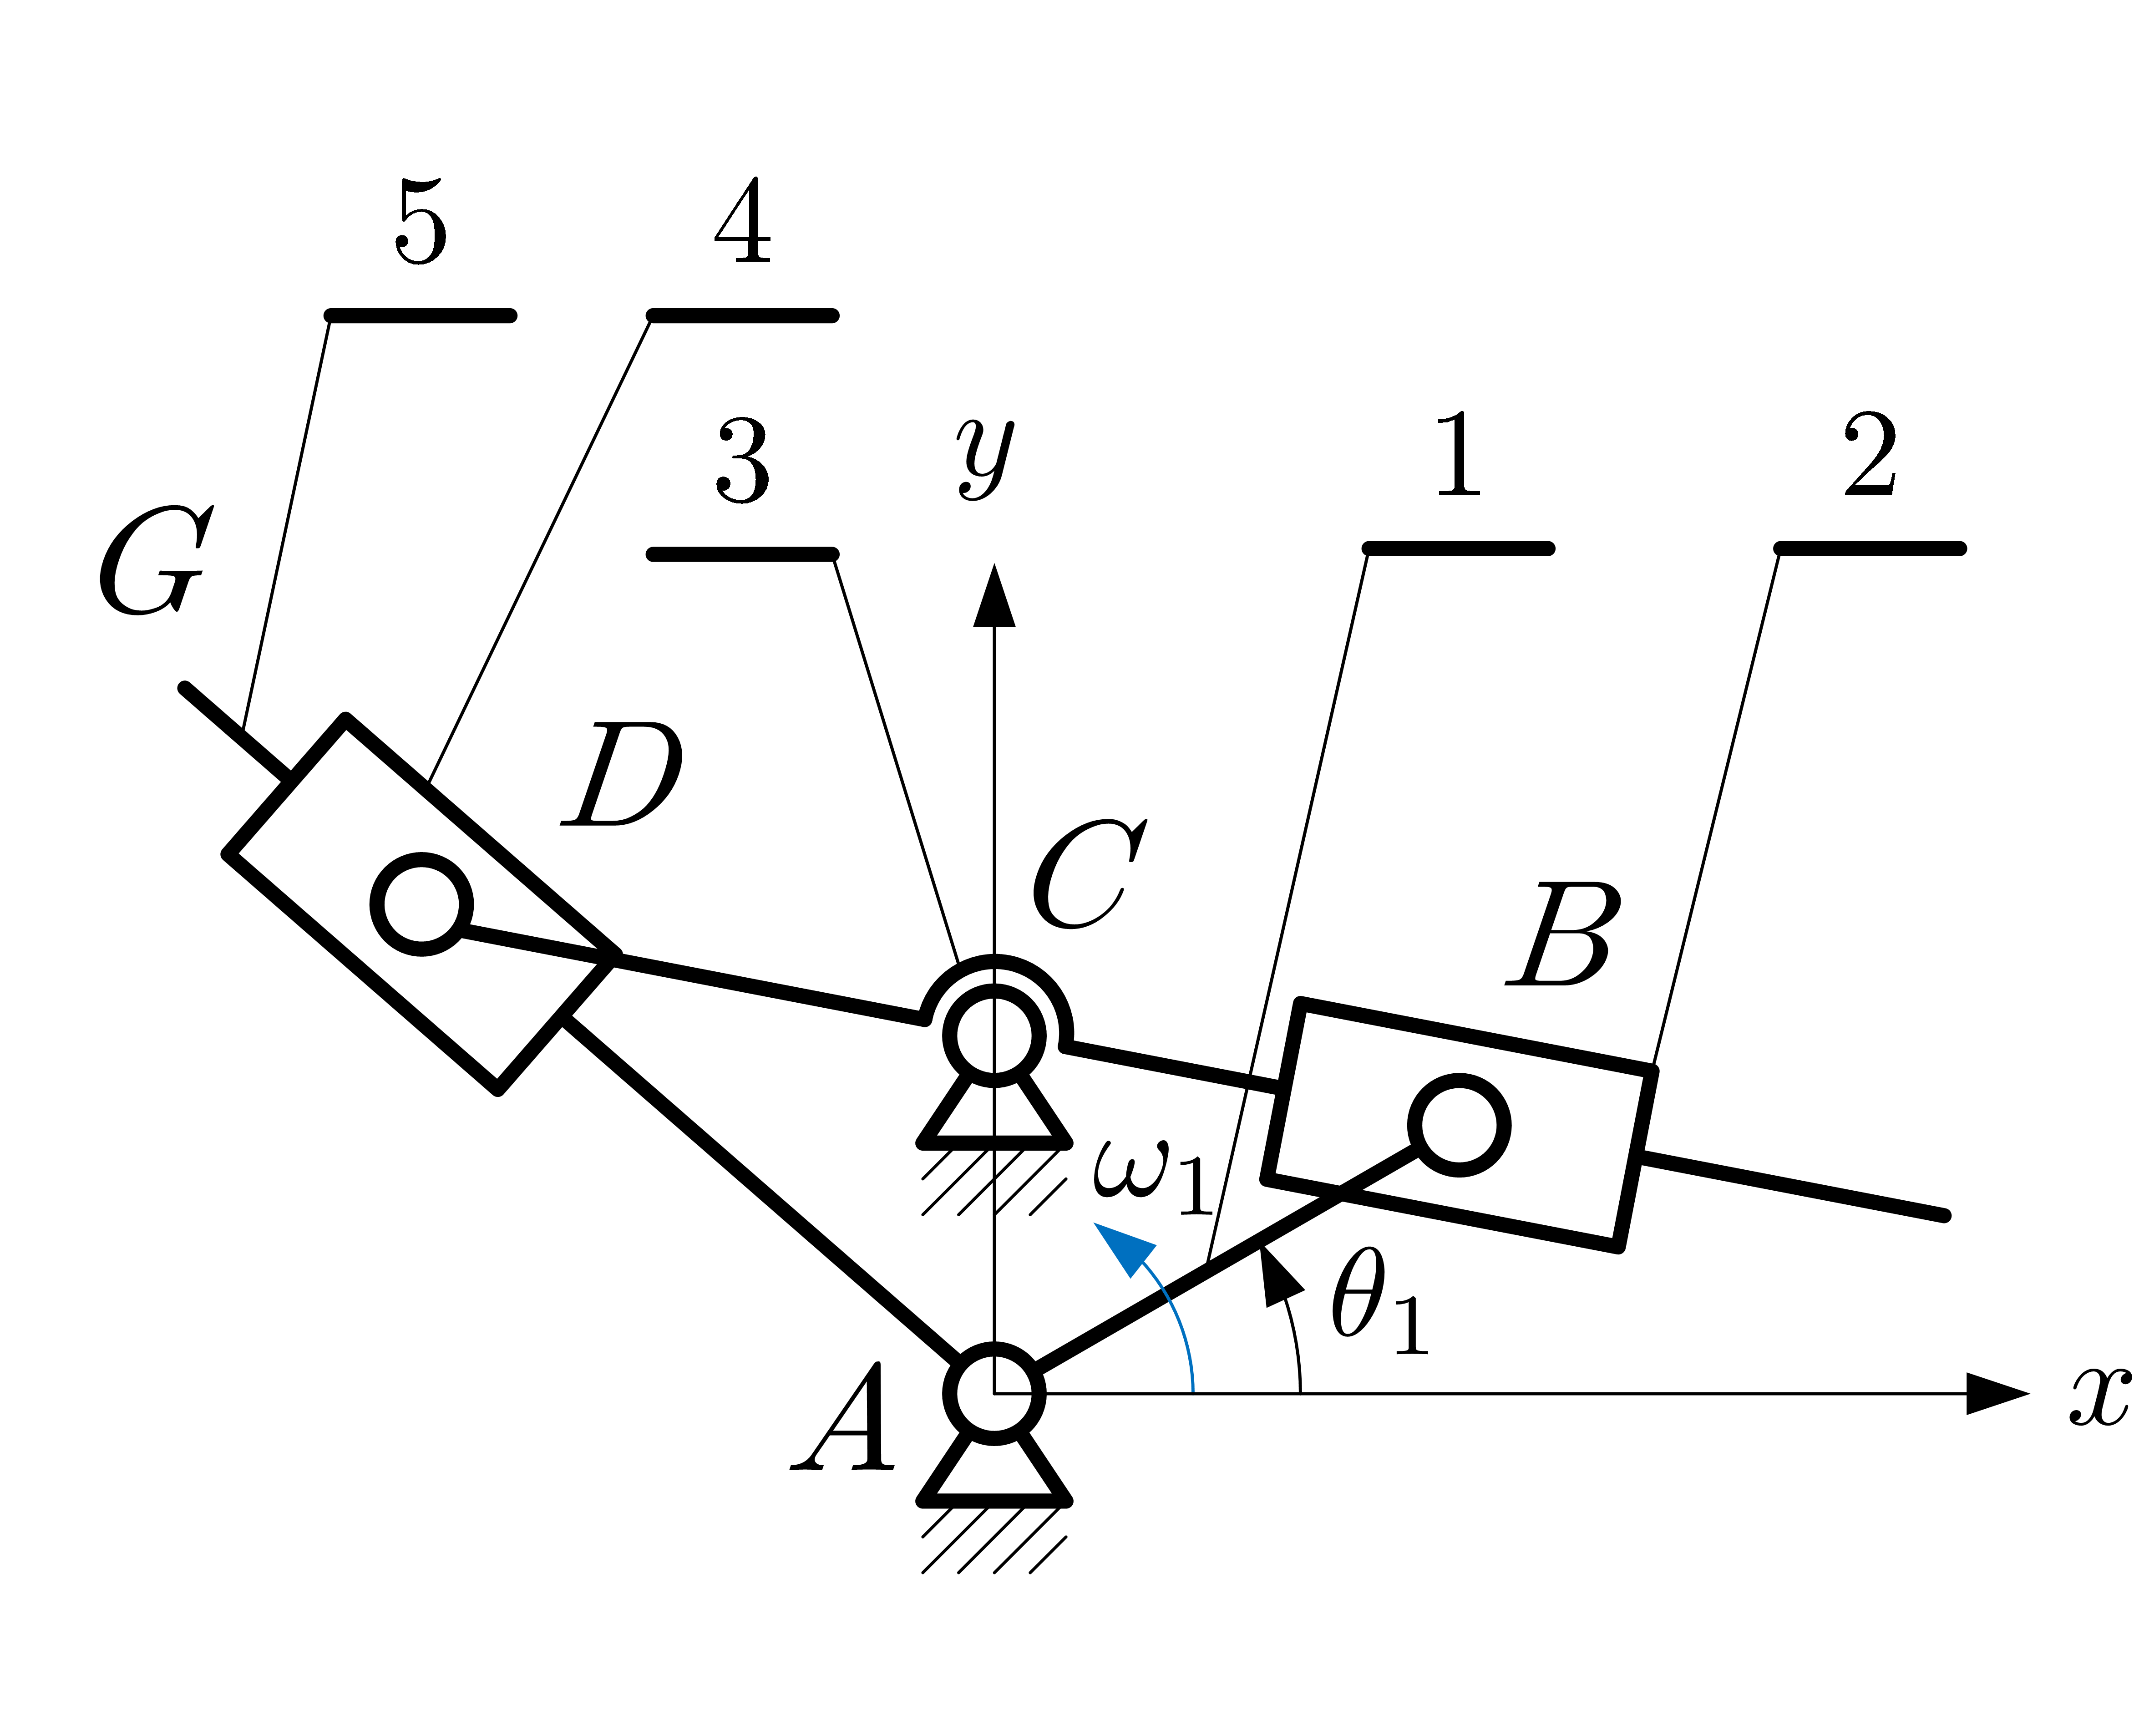
\includegraphics[width=55mm]{images/R-RTR-RTR.png}
				\end{figure}
			\end{minipage}
		\end{table}	
	\end{block}
\emph{Solution}\vskip2.5mm
Position of joint B:  $\displaystyle \vb{r}{B} = x_B\ih + y_B\jh = l_1\cos{\theta_1}\ih + l_1\sin{\theta_1}\jh$\\
Position of joint C:  $\displaystyle \vb{r}{C} = x_C\ih + y_C\jh = 0.1\jh$\\
Position of joint D: $\displaystyle \vb{r}{D} = x_D\ih + y_D\jh$\\
\end{frame}

\begin{frame}
Position of joint E: $\displaystyle \vb{r}{E} = x_E\ih + y_E\jh$\\
Position of joint G: $\displaystyle \vb{r}{G} = x_G\ih + y_G\jh$

	\[\Rightarrow \begin{cases}
	x_D^2 + (y_D-x_C)^2 = l_3^2\\
	\displaystyle \frac{y_D-y_C}{x_D-x_C} = \frac{y_D-y_B}{x_D-x_B}
	\end{cases} \]
	
	Solving the system of equations yields $x_{D_1}$ and $x_{D_2}$. Since $\theta_1\in [0,90)$, the condition is $x_D\leq x_C$
	
	\[\Rightarrow\begin{cases}
	\displaystyle \theta_2=\arctan{\frac{y_B-y_C}{x_B-x_C}}\\
	\displaystyle\theta_3=\theta_2\\
	\displaystyle\theta_4=\arctan{\frac{y_D}{x_D}}\\
	\displaystyle\theta_5=\theta_4
	\end{cases}\]

For other an arbitrary angle $\theta_1$, finding the right condition is tricky (\textit{4 conditions} corresponding to 4 quadrants of 1 full rotation).
\end{frame}

\begin{frame}
	\begin{table}
		\centering
		\begin{tabular}{l|l|l|l}
			$1^{st}$ quadrant & $2^{nd}$ quadrant & $3^{rd}$ quadrant & $4^{th}$ quadrant \\\hline
			$x_D\leq x_C=0$   & $x_D\geq x_C=0$   & $x_D\geq x_C=0$   & $x_D\leq x_C=0$
		\end{tabular}
		\caption{4 conditions to find $x_D$ from $[0,2\pi]$}
	\end{table}

	For this mechanism, observe that for any $\theta_1$:
	
	\begin{itemize}
		\item $x_Dx_B<0$
		\item $\vb{r}{{DC}}$ and $\vb{r}{{DF}}$ have the same angle 
		\item $\vb{r}{D}$ and $\vb{r}{G}$ have the same angle
	\end{itemize}

	Using these properties, we can obtain direct solution of position analysis for the mechanism:\\
	
	\begin{itemize}
		\item Find $\vb{r}{D}$
		\[\begin{cases}
		\displaystyle\langle \vb{Ox},\vb{r}{CD}\rangle = \arctan{\frac{y_B-y_C}{x_B-x_C}} + \pi\\
		\displaystyle\vb{r}{D} = \vb{r}{C} + sign(x_B)l_3\left(\cos{\langle\vb{Ox},\vb{r}{CD}\rangle}\ih + \sin{\langle \vb{Ox},\vb{r}{CD}\rangle}\jh\right)
		\end{cases}\]
	\end{itemize}
\end{frame}

\begin{frame}
	\begin{itemize}
		\item Find $\vb{r}{F}$
		\[\begin{cases}
		\displaystyle \langle \vb{Ox}, \vb{r}{FC}\rangle = \arctan{\frac{y_C-y_D}{x_C-x_D}}\\
		\displaystyle\vb{r}{F} = \vb{r}{C}+sign(x_B)(l_4-l_3)\left(\cos{\langle \vb{Ox},\vb{r}{FC}\rangle\ih} + \sin{\langle \vb{Ox},\vb{r}{FC}\rangle\jh}\right)
		\end{cases}\]
		\item Find $\vb{r}{G}$
		\[\begin{cases}
		\displaystyle \langle \vb{Ox}, \vb{r}{G}\rangle = \arctan{\frac{y_D}{x_D}}\\
		\displaystyle\vb{r}{G} = -sign(x_B)l_5\left(\cos{\langle \vb{Ox},\vb{r}{G}\rangle\ih}+\sin{\langle \vb{Ox},\vb{r}{G}\rangle\jh}\right)
		\end{cases}\]
	\end{itemize}
Note that $\arctan{\theta}\in(-\frac{\pi}{2}, \frac{\pi}{2})$, which leads to the presence of $sign(x_B)$.
\end{frame}


\begin{frame}{MATLAB R2019a code}
\lstinputlisting[style=Matlab-editor, basicstyle=\mlttfamily]{codes/RRTRRTR-position01.m}
\end{frame}

\begin{frame}{MATLAB R2019a code}
\lstinputlisting[style=Matlab-editor, basicstyle=\mlttfamily]{codes/RRTRRTR-position02.m}
\end{frame}
\begin{frame}{MATLAB R2019a code (direct solution)}
	\lstinputlisting[style=Matlab-editor, basicstyle=\mlttfamily]{codes/RRTRRTR-position1.m}
\end{frame}
\begin{frame}{MATLAB R2019a code (direct solution)}
\lstinputlisting[style=Matlab-editor, basicstyle=\mlttfamily]{codes/RRTRRTR-position2.m}
\end{frame}
\begin{frame}{Plotting using MATLAB R2019a}
\lstinputlisting[style=Matlab-editor, basicstyle=\mlttfamily]{codes/RRTRRTR-plot.m}
\end{frame}
\begin{frame}{Output figure}
\centering
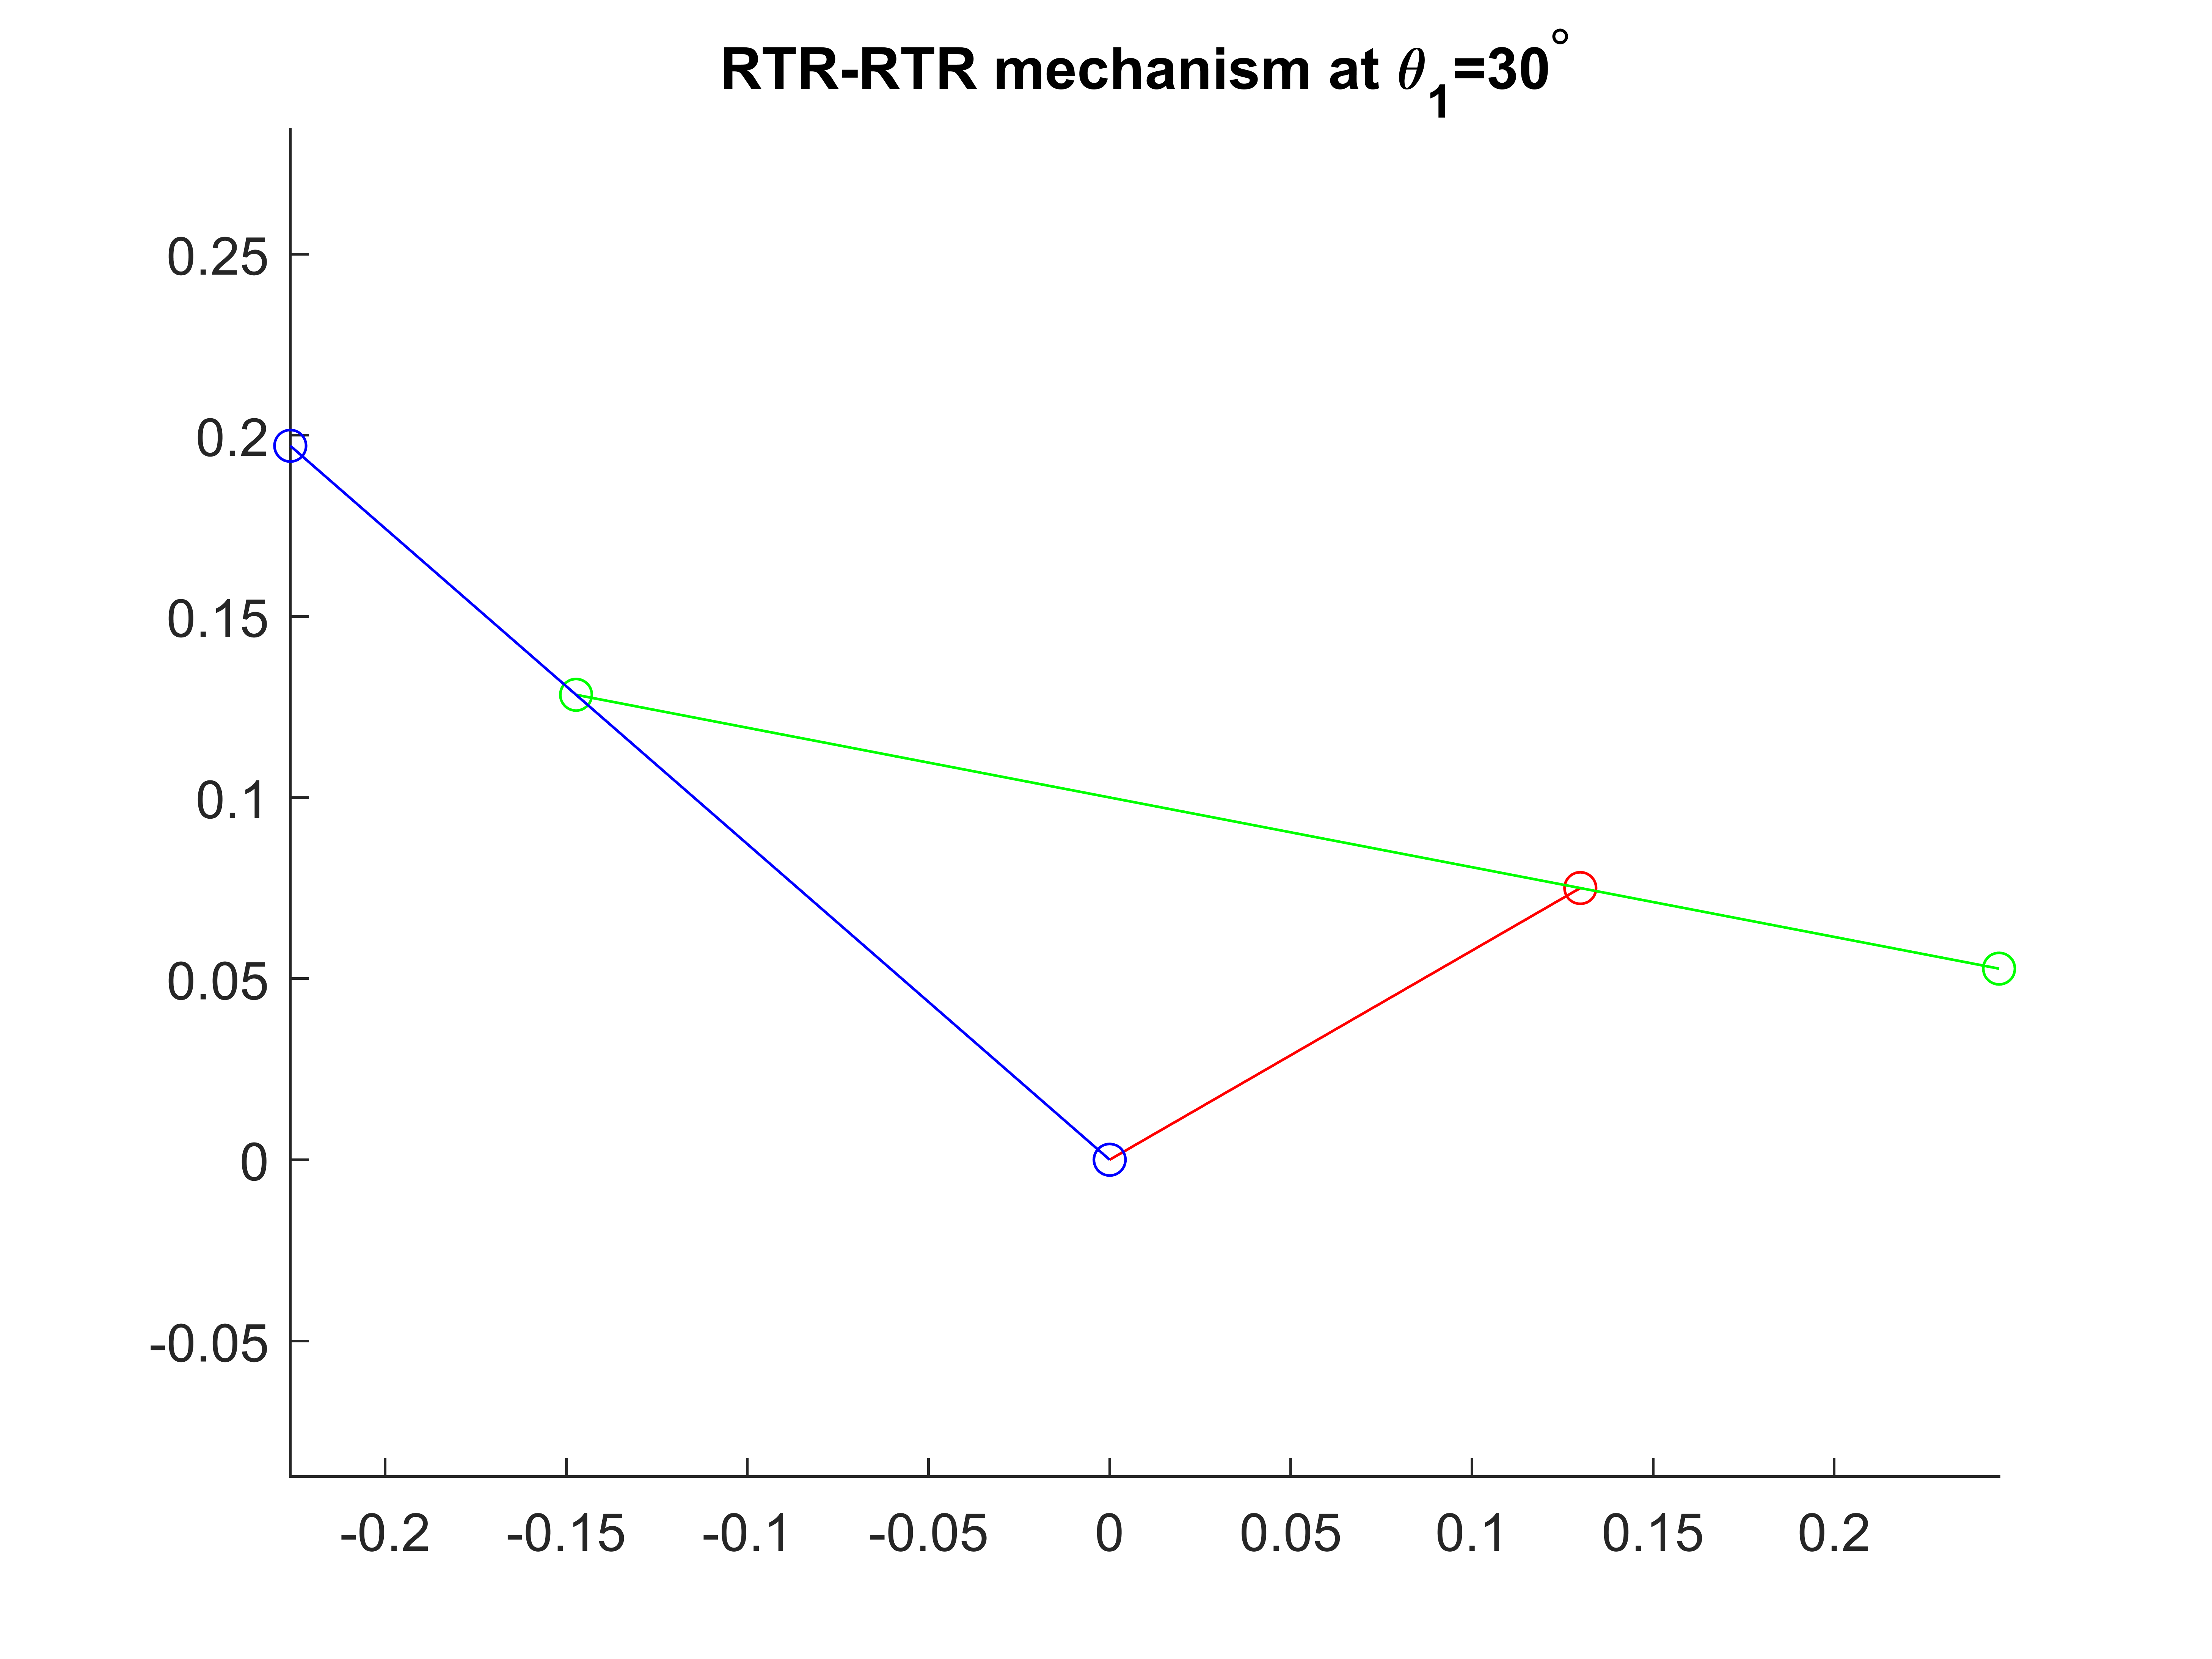
\includegraphics[width=100mm]{images/RRTRRTR-plot.png}
\end{frame}
\begin{frame}{Trajectory plotting using MATLAB R2019a}
\lstinputlisting[style=Matlab-editor, basicstyle=\mlttfamily]{codes/RRTRRTR-trajectory.m}
\end{frame}
\begin{frame}{Output figure}
\centering
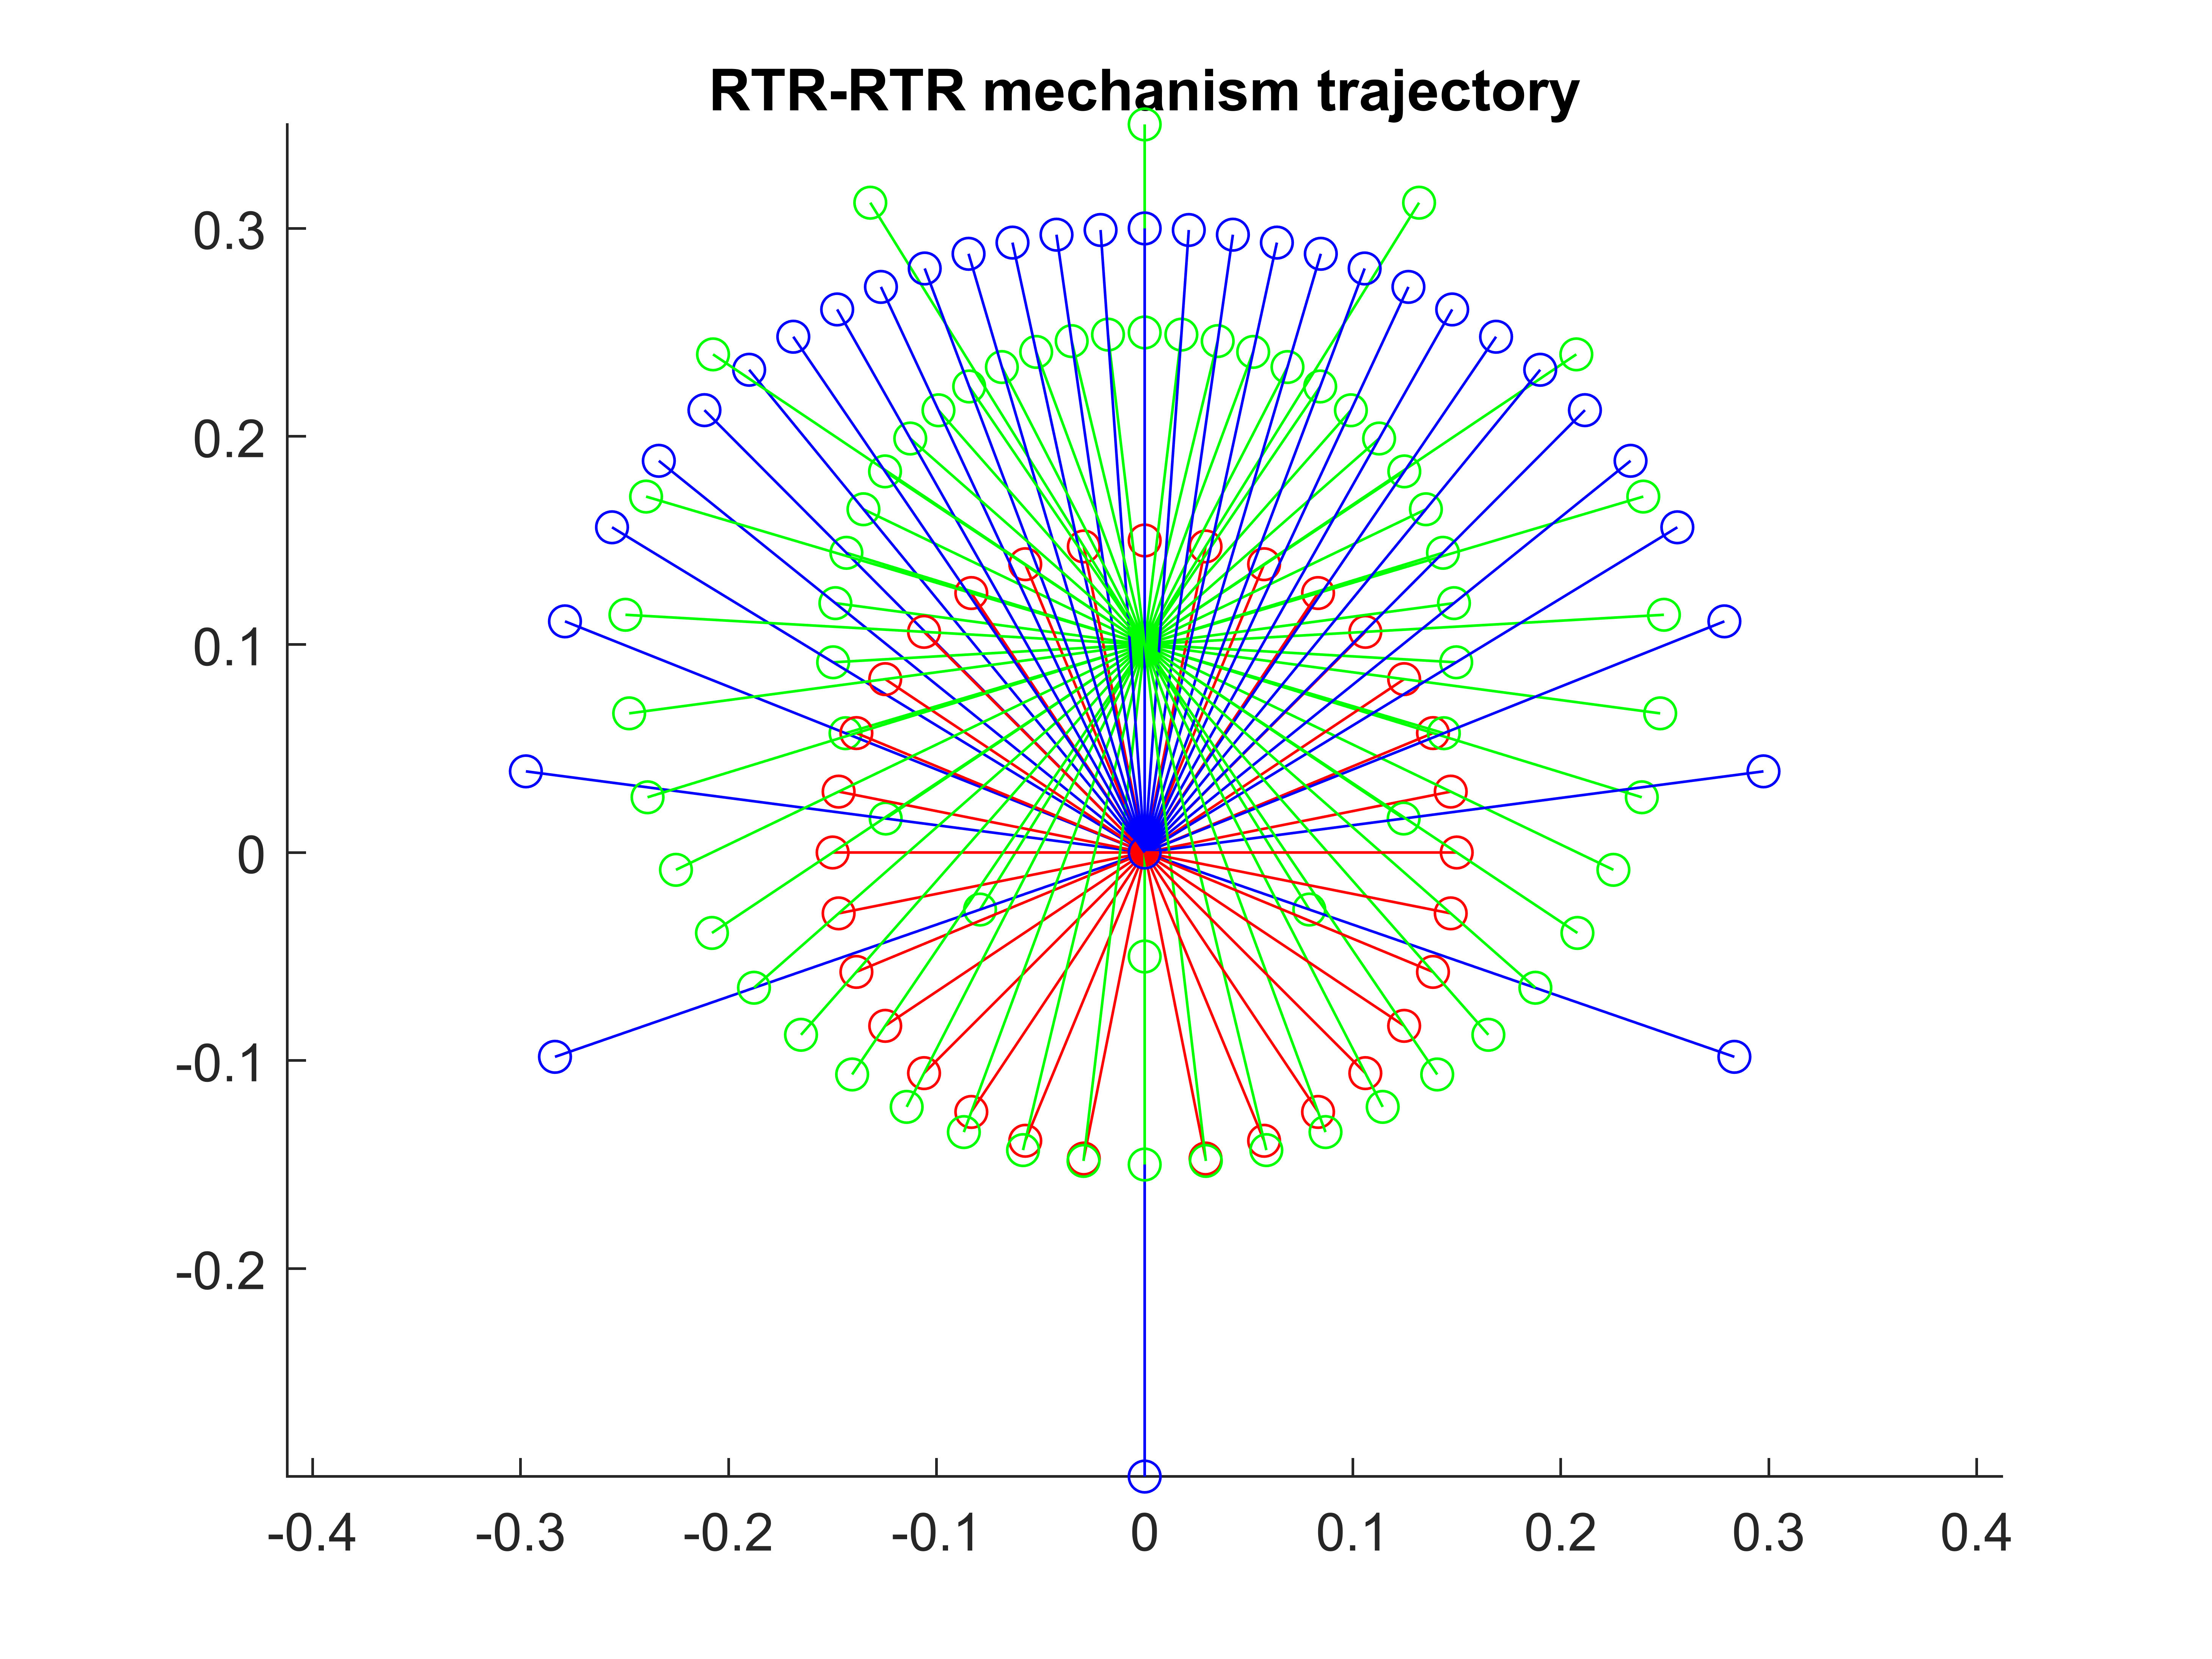
\includegraphics[width=100mm]{images/RRTRRTR-trajectory.png}
\end{frame}
